% chapter14.tex - 数值相对论简介
\chapter{数值相对论简介 (Introduction to Numerical Relativity)}
\label{chap:numerical_relativity}

数值相对论是用数值方法求解爱因斯坦场方程的学科。由于场方程的高度非线性，绝大多数天体物理上重要的强场动力学过程——如双黑洞并合、超新星核坍缩——没有解析解，必须借助大型计算机进行数值模拟。本章介绍数值相对论的基本框架：3+1分解（ADM形式）、BSSN演化系统、黑洞奇点处理以及引力波形提取技术。本章的主要参考文献包括 \cite{Gourgoulhon2007,Carroll1997,Wald1984}。

%=============================================================================
\section{为什么需要数值相对论？}
\label{sec:why_numerical_relativity}

爱因斯坦场方程是一组十个非线性耦合偏微分方程：
\begin{equation}
    G_{\mu\nu} + \Lambda g_{\mu\nu} = \frac{8\pi G}{c^4} T_{\mu\nu},
    \label{eq:Einstein_full}
\end{equation}
其中 $G_{\mu\nu}$ 是 Einstein 张量，它包含度规的二阶非线性项。非线性意味着：两个已知解的叠加\\
	extbf{不是}一个新解——强场区域的动力学行为极其复杂。

解析解（如 Schwarzschild 解、Kerr 解）仅存在于高度对称的稳态时空中。但在以下情况下，解析方法完全失效，必须依赖数值模拟：

\begin{enumerate}
    \item \textbf{双黑洞/双中子星并合}：两个致密天体相互绕转、在最后几圈剧烈加速、碰撞并合成一个天体。并合阶段的动力学是高度非线性的，辐射的引力波携带关于强场区域的丰富信息。
    \item \textbf{超新星核坍缩}：大质量恒星铁核坍缩为中子星或黑洞的过程涉及极端密度（$>10^{14}\,\text{g/cm}^3$）、强引力场和复杂的微观物理（中微子输运、状态方程），必须耦合广义相对论流体力学方程求解。
    \item \textbf{引力波天文学}：LIGO/Virgo/KAGRA 探测到的引力波信号（如 GW150914）需要精确的数值波形模板来匹配滤波和参数估计。有效单体理论（EOB）和唯象模型都需要数值相对论波形的校准。
    \item \textbf{宇宙学与早期宇宙}：某些暴胀模型中的非线性动力学（如 preheating 阶段）、拓扑缺陷（宇宙弦）的演化也需要数值相对论方法。
\end{enumerate}

\begin{note}[数值相对论的历史里程碑]
    \begin{itemize}
        \item 1960s：Arnowitt、Deser 和 Misner (ADM) 建立 3+1 分解的哈密顿形式 \cite{Wald1984}。
        \item 1990s：BSSN (Baumgarte--Shapiro--Shibata--Nakamura) 重新构造演化方程，解决了 ADM 形式的数值不稳定问题。
        \item 2005：Pretorius 首次完成双黑洞并合的完整数值模拟（使用广义调和坐标）。
        \item 2006：Campanelli 等人和 Baker 等人用 moving puncture 方法独立完成双黑洞并合模拟。
        \item 至今：数值相对论已成为引力波天文学的基石，提供精度达到 $<1\%$ 的波形模板。
    \end{itemize}
\end{note}

%=============================================================================
\section{3+1 分解：ADM 形式}
\label{sec:3plus1_ADM}

\subsection{时空的叶层结构}

3+1 分解的基本思想是将四维时空 $(\M, g_{\mu\nu})$ “切片”为一族三维类空超曲面 $\Sigma_t$（$t = \text{常数}$），然后研究这些超曲面的几何如何随时间演化。这与哈密顿力学中将时间分离出来处理动力学的方法一脉相承。

\begin{definition}[时空的叶层化 (Foliation)]
设 $\M$ 是全局双曲的时空流形。存在一个光滑的标量函数 $t: \M \to \mathbb{R}$，使得每个等值面
\begin{equation}
    \Sigma_t \equiv \{ p \in \M \mid t(p) = t \}
\end{equation}
是类空超曲面。这些 $\Sigma_t$ 的集合构成 $\M$ 的一个\textbf{叶层化}。每个 $\Sigma_t$ 称为一张“切片”。
\label{def:foliation}
\end{definition}

\begin{figure}[htbp]
\centering
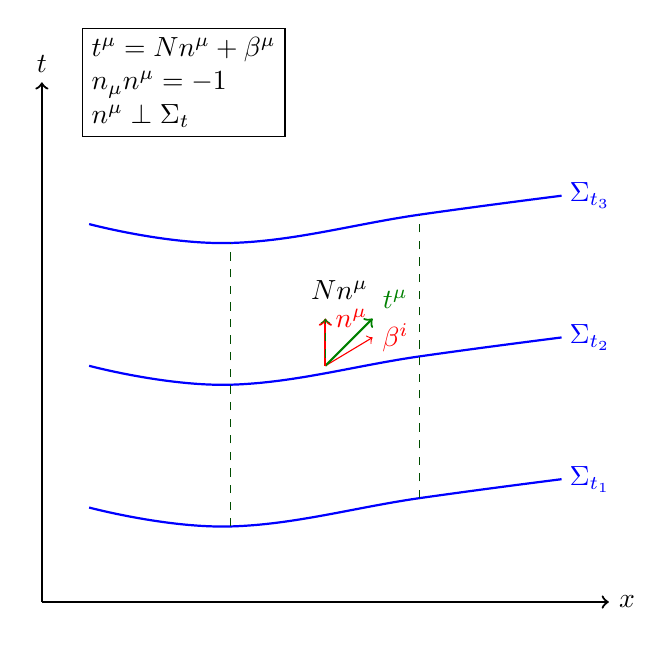
\begin{tikzpicture}[scale=1.2]
    % 坐标轴
    \draw[->,thick] (0,0) -- (6,0) node[right] {$x$};
    \draw[->,thick] (0,0) -- (0,5.5) node[above] {$t$};
    
    % 三张超曲面 \Sigma_{t1}, \Sigma_{t2}, \Sigma_{t3}
    \draw[blue,thick] plot[smooth,tension=0.7] coordinates {(0.5,1) (2,0.8) (4,1.1) (5.5,1.3)};
    \node[blue] at (5.8,1.3) {$\Sigma_{t_1}$};
    
    \draw[blue,thick] plot[smooth,tension=0.7] coordinates {(0.5,2.5) (2,2.3) (4,2.6) (5.5,2.8)};
    \node[blue] at (5.8,2.8) {$\Sigma_{t_2}$};
    
    \draw[blue,thick] plot[smooth,tension=0.7] coordinates {(0.5,4) (2,3.8) (4,4.1) (5.5,4.3)};
    \node[blue] at (5.8,4.3) {$\Sigma_{t_3}$};
    
    % 法向量 n (从 Sigma_{t2} 向上)
    \draw[red,->,thick] (3,2.5) -- (3,3.0) node[right] {$n^\mu$};
    \draw[red,->] (3,2.5) -- (3.5,2.8) node[right] {$\beta^i$};
    
    % 时间演化向量 t^mu
    \draw[->,thick,green!50!black] (3,2.5) -- (3.5,3.0) node[above right] {$t^\mu$};
    \draw[green!50!black,->] (3,2.5) -- (3,3.0);
    
    % 标注 N n
    \draw[red,dashed] (3,2.5) -- (3,3.0);
    \node at (3.15,3.3) {$N n^\mu$};
    
    % 世界线
    \draw[green!30!black,dashed] (2,0.8) -- (2,2.3) -- (2,3.8);
    \draw[green!30!black,dashed] (4,1.1) -- (4,2.6) -- (4,4.1);
    
    % 图例
    \node[draw,fill=white,align=left] at (1.5,5.5) {
        $t^\mu = N n^\mu + \beta^\mu$\\
        $n_\mu n^\mu = -1$\\
        $n^\mu \perp \Sigma_t$
    };
\end{tikzpicture}
\caption{3+1 分解的几何图示。时空被类空超曲面 $\Sigma_t$ 叶层化。$n^\mu$ 是 $\Sigma_t$ 的单位类时法向量。时间演化矢量 $t^\mu$ 分解为法向部分（lapse $N n^\mu$）和切向部分（shift $\beta^\mu$）。}
\label{fig:foliation}
\end{figure}

\subsection{Lapse 与 Shift}

叶层化引入了两个关键的运动学量：

\begin{definition}[Lapse 函数 $N$ 与 Shift 矢量 $\beta^i$]
设 $t^\mu = (\pd_t)^\mu$ 是坐标时间演化矢量。将 $t^\mu$ 相对于 $\Sigma_t$ 的法方向和切方向分解：
\begin{equation}
    \boxed{t^\mu = N n^\mu + \beta^\mu},
    \label{eq:lapse_shift_def}
\end{equation}
其中 $n^\mu$ 是 $\Sigma_t$ 的单位类时法向量（$n_\mu n^\mu = -1$），$\beta^\mu$ 是切向矢量（$\beta^\mu n_\mu = 0$），其空间分量记为 $\beta^i$。$N$ 称为\textbf{lapse 函数}，$\beta^i$ 称为\textbf{shift 矢量}。
\label{def:lapse_shift}
\end{definition}

Lapse 函数 $N$ 的物理含义：在相邻的两张时间切片之间，从一个切片上某一点出发，沿法向量 $n^\mu$ 方向行进的\textbf{固有时间}为 $\dd\tau = N \dd t$。因此 $N$ 描述了“时间流逝的速率”。

Shift 矢量 $\beta^i$ 的物理含义：它描述了空间坐标从一张切片到下一张切片时的“滑动”——即坐标系在空间方向上的漂移。

\subsection{四维度规的分解}

有了 lapse 和 shift，四维度规 $g_{\mu\nu}$ 可以用空间度规 $\gamma_{ij}$ 表示：

\begin{theorem}[ADM 度规分解]
在 3+1 分解下，四维线元写为：
\begin{equation}
    \boxed{\dd s^2 = -N^2 \dd t^2 + \gamma_{ij}(\dd x^i + \beta^i \dd t)(\dd x^j + \beta^j \dd t)}.
    \label{eq:ADM_line_element}
\end{equation}
或者等价地，四维度规及其逆为：
\begin{align}
    g_{\mu\nu} &= \begin{pmatrix}
        -N^2 + \beta_k\beta^k & \beta_i \\
        \beta_j & \gamma_{ij}
    \end{pmatrix},
    \label{eq:ADM_metric_matrix}
    \\[4pt]
    g^{\mu\nu} &= \begin{pmatrix}
        -1/N^2 & \beta^i/N^2 \\[2pt]
        \beta^j/N^2 & \gamma^{ij} - \beta^i\beta^j/N^2
    \end{pmatrix},
    \label{eq:ADM_inverse_metric}
\end{align}
其中 $\beta_i = \gamma_{ij}\beta^j$，$\beta_k\beta^k = \gamma_{ij}\beta^i\beta^j$。
\label{thm:ADM_metric}
\end{theorem}

\begin{proof}[推导]
由 $t^\mu = N n^\mu + \beta^\mu$，且 $n_\mu n^\mu = -1$，$n_\mu \beta^\mu = 0$。四维线元 $\dd s^2 = g_{\mu\nu}\dd x^\mu\dd x^\nu$，其中 $\dd x^0 = \dd t$。将坐标微分写为 $\dd x^\mu = t^\mu \dd t + (\dd x^\mu)_\perp$，其中 $(\dd x^\mu)_\perp$ 是 $\Sigma_t$ 上的切矢量。经过直接计算可得式 (\ref{eq:ADM_line_element})。详细推导见 \cite{Gourgoulhon2007}。
\end{proof}

\begin{note}[符号约定]
本书中，四维时空指标为希腊字母 ($\mu,\nu,\ldots=0,1,2,3$)，三维空间指标为拉丁字母 ($i,j,\ldots=1,2,3$)。空间度规 $\gamma_{ij}$ 是正定的。$\gamma^{ij}$ 是 $\gamma_{ij}$ 的逆：$\gamma^{ik}\gamma_{kj} = \delta^i_j$。
\end{note}

%=============================================================================
\section{诱导度规与外曲率}
\label{sec:induced_extrinsic}

\subsection{诱导度规 $\gamma_{ij}$}

类空超曲面 $\Sigma_t$ 从四维时空度规继承了一个\textbf{诱导度规}（induced metric）——也称为\textbf{第一基本形式}：

\begin{definition}[诱导度规 / 空间度规]
$\Sigma_t$ 上的诱导度规 $\gamma_{ij}$ 定义为四维度规 $g_{\mu\nu}$ 在 $\Sigma_t$ 上的限制：
\begin{equation}
    \boxed{\gamma_{ij} \equiv g_{\mu\nu} \, e^\mu_i \, e^\nu_j},
    \label{eq:gamma_def}
\end{equation}
其中 $e^\mu_i = \pd x^\mu / \pd y^i$ 是将 $\Sigma_t$ 上的坐标 $y^i$ 映射到时空坐标 $x^\mu$ 的切映射。在实际计算中，通常取 $y^i = x^i$（空间坐标），此时 $\gamma_{ij}$ 恰好就是四维度规的空间分量。
\end{definition}

度规 $\gamma_{ij}$ 的协变导数记为 $D_i$（与四维协变导数 $\nabla_\mu$ 区分）。相应的三维 Christoffel 符号为：
\begin{equation}
    \Gamma^i_{jk} = \frac{1}{2}\gamma^{i\ell}(\pd_j\gamma_{k\ell} + \pd_k\gamma_{j\ell} - \pd_\ell\gamma_{jk}).
    \label{eq:Gamma3}
\end{equation}

\subsection{外曲率 $K_{ij}$}

除了度规，$\Sigma_t$ 作为嵌入在四维时空中的超曲面还有第二个基本微分几何量——\textbf{外曲率}（extrinsic curvature，第二基本形式）：

\begin{definition}[外曲率]
$\Sigma_t$ 的外曲率 $K_{\mu\nu}$ 定义为法向量 $n^\mu$ 的协变导数在 $\Sigma_t$ 上的投影：
\begin{equation}
    \boxed{K_{\mu\nu} \equiv -\gamma^\rho_\mu \gamma^\sigma_\nu \nabla_\rho n_\sigma}.
    \label{eq:K_def}
\end{equation}
其中 $\gamma^\mu_\nu = \delta^\mu_\nu + n^\mu n_\nu$ 是投影到 $\Sigma_t$ 上的投影算子。外曲率的空间分量记为 $K_{ij}$。
\label{def:extrinsic_curvature}
\end{definition}

外曲率也可以理解为法向量沿 $\Sigma_t$ 的 Lie 导数的负数：
\begin{equation}
    K_{ij} = -\frac{1}{2}\Lie_n \gamma_{ij},
    \label{eq:K_Lie}
\end{equation}
其中 $\Lie_n$ 是沿法向量 $n^\mu$ 的李导数。由此得到 $K_{ij}$ 的运动学表达式：
\begin{equation}
    \boxed{K_{ij} = \frac{1}{2N}\left(D_i\beta_j + D_j\beta_i - \pd_t\gamma_{ij}\right)}.
    \label{eq:K_kinematic}
\end{equation}

\begin{property}[外曲率的物理含义]
    \begin{enumerate}
        \item 外曲率描述 $\Sigma_t$ 如何嵌入在四维时空中的“弯曲程度”——即法向量沿超曲面的变化率。
        \item $K_{ij} = 0$ 意味着超曲面是“全测地的”（totally geodesic），即法向量沿超曲面保持不变。
        \item 迹 $K = \gamma^{ij}K_{ij}$ 称为\textbf{平均曲率}，描述空间体积元的膨胀率：$\dd V / \dd\tau = -K \dd V$。
        \item 在宇宙学中，$K = -3H$（Hubble 参数），负号源于我们的符号约定。
    \end{enumerate}
\end{property}

\subsection{Gauss--Codazzi 关系}

四维时空的曲率与三维超曲面上的几何量通过 Gauss--Codazzi 方程相关联：

\begin{theorem}[Gauss--Codazzi 方程]
四维 Riemann 张量 $R^\mu_{\nu\rho\sigma}$ 在 $\Sigma_t$ 上的投影可以分解为：
\begin{align}
    \boxed{\gamma^\mu_\alpha \gamma^\beta_\nu \gamma^\rho_\gamma \gamma^\sigma_\delta \, R^\alpha_{\beta\rho\sigma} = {}^{(3)}\!R^\mu_{\nu\gamma\delta} + K^\mu_\gamma K_{\nu\delta} - K^\mu_\delta K_{\nu\gamma}},
    \label{eq:Gauss}
\end{align}
这是\textbf{Gauss 方程}，其中 ${}^{(3)}\!R^\mu_{\nu\gamma\delta}$ 是由 $\gamma_{ij}$ 计算的三维 Riemann 张量。

\textbf{Codazzi 方程}将 Ricci 张量的混合投影与外曲率的三维协变导数相联系：
\begin{equation}
    \boxed{\gamma^\mu_\alpha \gamma^\rho_\beta n^\sigma \, R_{\mu\rho\nu\sigma} = D_\beta K_{\alpha\nu} - D_\alpha K_{\beta\nu}}.
    \label{eq:Codazzi}
\end{equation}
\label{thm:Gauss_Codazzi}
\end{theorem}

这些关系是将四维 Einstein 方程分解为约束方程和演化方程的关键工具。详细的推导可参阅 \cite{Gourgoulhon2007,Wald1984}。

%=============================================================================
\section{ADM 演化方程与约束方程}
\label{sec:ADM_evolution_constraints}

\subsection{约束方程}

将 Gauss--Codazzi 关系代入 Einstein 方程，可以得到两组不与时间导数有关的方程——即每张空间切片上都必须满足的\textbf{约束方程}（constraint equations）：

\begin{theorem}[Hamilton 约束方程]
由 Einstein 方程的 $G_{\mu\nu}n^\mu n^\nu = \frac{8\pi G}{c^4} T_{\mu\nu}n^\mu n^\nu$ 得到：
\begin{equation}
    \boxed{{}^{(3)}\!R + K^2 - K_{ij}K^{ij} = \frac{16\pi G}{c^4} \rho},
    \label{eq:Hamiltonian_constraint}
\end{equation}
其中 ${}^{(3)}\!R$ 是由 $\gamma_{ij}$ 计算的三维 Ricci 标量，$K = \gamma^{ij}K_{ij}$ 是平均曲率，$\rho \equiv T_{\mu\nu}n^\mu n^\nu$ 是 Euler 观测者测得的能量密度。
\label{thm:Hamiltonian_constraint}
\end{theorem}

\begin{theorem}[动量约束方程]
由 Einstein 方程的混合投影 $G_{\mu\nu}\gamma^\mu_\alpha n^\nu = \frac{8\pi G}{c^4} T_{\mu\nu}\gamma^\mu_\alpha n^\nu$ 得到：
\begin{equation}
    \boxed{D_j(K^{ij} - \gamma^{ij}K) = \frac{8\pi G}{c^4} j^i},
    \label{eq:momentum_constraint}
\end{equation}
其中 $j^i \equiv -T_{\mu\nu}\gamma^{i\mu}n^\nu$ 是动量密度。
\label{thm:momentum_constraint}
\end{theorem}

在真空中（$\rho=0, j^i=0$），约束方程简化为：
\begin{align}
    {}^{(3)}\!R + K^2 - K_{ij}K^{ij} &= 0, \label{eq:vacuum_Hamiltonian} \\
    D_j(K^{ij} - \gamma^{ij}K) &= 0. \label{eq:vacuum_momentum}
\end{align}

\begin{note}[约束方程的角色]
    约束方程不包含 $\gamma_{ij}$ 或 $K_{ij}$ 的时间导数——它们必须在\textbf{初始数据}上精确满足。如果初始数据满足约束，则演化方程保证约束在以后的各个时刻自动满足（这是 Bianchi 恒等式的结果）。在数值计算中，约束违反的增长是衡量数值精度的重要指标。
\end{note}

\subsection{演化方程}

$\gamma_{ij}$ 和 $K_{ij}$ 的时间演化由以下方程控制：

\begin{theorem}[ADM 演化方程]
空间度规的演化方程（本质上是 $K_{ij}$ 的定义式）：
\begin{equation}
    \boxed{\pd_t \gamma_{ij} = -2N K_{ij} + D_i\beta_j + D_j\beta_i}.
    \label{eq:ADM_evol_gamma}
\end{equation}

外曲率的演化方程（由 Einstein 方程的空间投影得到）：
\begin{equation}
    \boxed{\begin{aligned}
        \pd_t K_{ij} &= N\bigl({}^{(3)}\!R_{ij} - 2K_{ik}K^k_j + K K_{ij}\bigr) - D_i D_j N \\
        &\quad + \beta^k D_k K_{ij} + K_{ik}D_j\beta^k + K_{kj}D_i\beta^k \\
        &\quad - 4\pi G N\bigl(2S_{ij} - \gamma_{ij}(S - \rho)\bigr).
    \end{aligned}}
    \label{eq:ADM_evol_K}
\end{equation}
其中 $S_{ij} \equiv T_{\mu\nu}\gamma^\mu_i\gamma^\nu_j$ 是空间应力张量，$S = \gamma^{ij}S_{ij}$ 是其迹。
\label{thm:ADM_evolution}
\end{theorem}

完整的 ADM 动力学系统包括：六个 $\gamma_{ij}$ 演化方程、六个 $K_{ij}$ 演化方程，加上 Hamilton 约束和三个动量约束——一共是十二个演化变量和四个约束。Lapse $N$ 和 shift $\beta^i$ 不是动力学变量，而是\textbf{规范自由度}，可以自由选择（对应坐标条件的选取）。

\begin{note}[ADM 形式的数值困境]
    尽管 ADM 形式在理论上优雅完备，但在实际数值模拟中表现出严重的\textbf{数值不稳定性}。其根本原因在于 ADM 方程系统不是强双曲的（strongly hyperbolic），微小的高频噪声会在演化过程中迅速增长。这一难题直到 1990 年代 BSSN 重新构造演化方程后才得以解决。
\end{note}

%=============================================================================
\section{BSSN 形式}
\label{sec:BSSN}

由于 ADM 形式的数值不稳定性，Baumgarte、Shapiro、Shibata 和 Nakamura 在 1990 年代提出了一种重新构造的演化系统——\textbf{BSSN 形式}，现在已成为数值相对论的主流方案。

\subsection{共形分解}

BSSN 形式的核心思想是将空间度规进行共形分解：

\begin{definition}[BSSN 变数]
引入共形因子 $\phi$ 或 $\chi$，将空间度规分解为：
\begin{equation}
    \boxed{\gamma_{ij} = e^{4\phi} \tilde{\gamma}_{ij} \quad\text{或}\quad \gamma_{ij} = \chi^{-1}\tilde{\gamma}_{ij}},
    \label{eq:conformal_decomp}
\end{equation}
其中 $\tilde{\gamma}_{ij}$ 是\textbf{共形度规}，其行列式被固定（通常取 $\det\tilde{\gamma}_{ij} = 1$，从而 $\chi = (\det\gamma_{ij})^{-1/3} = e^{-4\phi}$）。

外曲率分解为迹部分和无迹部分：
\begin{align}
    K &= \gamma^{ij}K_{ij}, \label{eq:trace_K} \\
    \tilde{A}_{ij} &\equiv e^{-4\phi}\left(K_{ij} - \frac{1}{3}\gamma_{ij}K\right),
    \label{eq:Atilde_def}
\end{align}
使得 $\tilde{A}_{ij}$ 对共形度规无迹：$\tilde{\gamma}^{ij}\tilde{A}_{ij} = 0$。
\label{def:BSSN_variables}
\end{definition}

此外，引入\textbf{共形联络函数}（conformal connection functions）：
\begin{equation}
    \boxed{\tilde{\Gamma}^i \equiv \tilde{\gamma}^{jk}\tilde{\Gamma}^i_{jk} = -\pd_j \tilde{\gamma}^{ij}},
    \label{eq:Gamma_conformal}
\end{equation}
其中 $\tilde{\Gamma}^i_{jk}$ 是由共形度规 $\tilde{\gamma}_{ij}$ 计算的 Christoffel 符号。$\tilde{\Gamma}^i$ 在 BSSN 中被提升为独立的演化变量，这是使系统强双曲的关键步骤。

\subsection{BSSN 演化方程}

BSSN 系统的完整演化方程如下（真空中，$c=1, G=1$）：

\begin{theorem}[BSSN 演化系统]
\textbf{共形因子：}
\begin{equation}
    \pd_t \phi = -\frac{1}{6}N K + \beta^i\pd_i\phi + \frac{1}{6}\pd_i\beta^i.
    \label{eq:BSSN_phi}
\end{equation}

\textbf{共形度规：}
\begin{equation}
    \pd_t \tilde{\gamma}_{ij} = -2N\tilde{A}_{ij} + \beta^k\pd_k\tilde{\gamma}_{ij} + \tilde{\gamma}_{ik}\pd_j\beta^k + \tilde{\gamma}_{kj}\pd_i\beta^k - \frac{2}{3}\tilde{\gamma}_{ij}\pd_k\beta^k.
    \label{eq:BSSN_gammatilde}
\end{equation}

\textbf{外曲率迹：}
\begin{equation}
    \pd_t K = -\gamma^{ij}D_i D_j N + N\left(\tilde{A}_{ij}\tilde{A}^{ij} + \frac{1}{3}K^2\right) + \beta^i\pd_i K.
    \label{eq:BSSN_K}
\end{equation}

\textbf{无迹外曲率：}
\begin{equation}
    \begin{aligned}
        \pd_t \tilde{A}_{ij} &= e^{-4\phi}\Bigl[-D_i D_j N + N\,{}^{(3)}\!R_{ij}\Bigr]^{\text{TF}} \\
        &\quad + N\left(K\tilde{A}_{ij} - 2\tilde{A}_{ik}\tilde{A}^k_j\right) \\
        &\quad + \beta^k\pd_k\tilde{A}_{ij} + \tilde{A}_{ik}\pd_j\beta^k + \tilde{A}_{kj}\pd_i\beta^k - \frac{2}{3}\tilde{A}_{ij}\pd_k\beta^k,
    \end{aligned}
    \label{eq:BSSN_Atilde}
\end{equation}
其中 $[\cdots]^{\text{TF}}$ 表示取无迹部分。

\textbf{共形联络函数：}
\begin{equation}
    \begin{aligned}
        \pd_t \tilde{\Gamma}^i &= -2\tilde{A}^{ij}\pd_j N + 2N\Bigl(\tilde{\Gamma}^i_{jk}\tilde{A}^{kj} - \frac{2}{3}\tilde{\gamma}^{ij}\pd_j K\Bigr) \\
        &\quad + \beta^j\pd_j\tilde{\Gamma}^i - \tilde{\Gamma}^j\pd_j\beta^i + \frac{2}{3}\tilde{\Gamma}^i\pd_j\beta^j + \tilde{\gamma}^{jk}\pd_j\pd_k\beta^i.
    \end{aligned}
    \label{eq:BSSN_Gamma}
\end{equation}
\label{thm:BSSN_system}
\end{theorem}

\begin{property}[BSSN vs ADM]
    BSSN 系统相比 ADM 的优越之处：
    \begin{enumerate}
        \item \textbf{强双曲性}：将 $\tilde{\Gamma}^i$ 提升为独立变量后，演化系统的主部具有强双曲结构，保证适定性（well-posedness）。
        \item \textbf{约束传播}：约束方程（Hamilton 和动量约束）的违反在 BSSN 中不会自发增长——系统具有“约束阻尼”性质。
        \item \textbf{共形分解}：将体积因子（共形因子 $\phi$ 或 $\chi$）与形状（共形度规 $\tilde{\gamma}_{ij}$）分离，使奇点附近的数值行为更可控。
    \end{enumerate}
\end{property}

\subsection{规范条件}

Lapse 和 shift 的选择（即\textbf{切片条件}和\textbf{空间坐标条件}）对数值模拟的稳定性和物理结果至关重要。BSSN 常用的规范条件有：

\begin{definition}[1+log 切片条件]
\begin{equation}
    \boxed{\pd_t N = \beta^i \pd_i N - 2 N K}.
    \label{eq:one_plus_log}
\end{equation}
这个条件使得 $N$ 沿法向量的 Lie 导数为 $\Lie_n N = -2K$。在 $K>0$（坍缩）区域，$N$ 减小（时间“冻结”），这对黑洞奇点附近的模拟极其有利——称为\textbf{奇点避免切片}（singularity-avoiding slicing）。
\label{def:one_plus_log}
\end{definition}

\begin{definition}[Gamma-driver 条件]
Shift 矢量 $\beta^i$ 的演化通常由\textbf{Gamma-driver} 条件控制：
\begin{align}
    \pd_t \beta^i &= \frac{3}{4} B^i, \label{eq:gamma_driver1} \\
    \pd_t B^i &= \pd_t \tilde{\Gamma}^i - \eta B^i,
    \label{eq:gamma_driver2}
\end{align}
其中 $\eta$ 是阻尼参数（典型的取值 $\eta \sim 1/(2M)$）。这个条件使 $\tilde{\Gamma}^i$ 趋近于零，从而保持空间坐标的“最小畸变”状态。
\label{def:gamma_driver}
\end{definition}

\begin{note}[移动 puncture 方法]
1+log 切片与 Gamma-driver 条件的组合构成了著名的\textbf{移动 puncture 方法}（moving puncture method）的核心。这一方法不需要对黑洞内部进行特殊的奇点切除（excision），而是在奇点附近自然地“冻结”演化，使数值模拟能够稳定地穿越视界。搭配 BSSN 演化系统，移动 puncture 方法是目前应用最广泛的黑洞并合数值方案。
\end{note}

%=============================================================================
\section{黑洞模拟中的奇点处理}
\label{sec:singularity_treatment}

黑洞时空中存在物理奇点（曲率发散处）。如何在数值模拟中处理奇点而不使计算崩溃，是数值相对论中的核心工程问题。有三种主要策略：

\subsection{Puncture 方法}

Puncture 方法是处理黑洞初始数据的一种技术。

\begin{definition}[Puncture 初始数据]
在 Brill--Lindquist 类型的初始数据中，黑洞由 Schwarzschild 时空的 Einstein--Rosen 桥（wormhole）的“喉咙”表示。通过共形分解，在坐标奇点（puncture）附近，共形因子以 $\phi \sim \ln r$（或 $\chi \sim r^2$）的行为发散。在数值网格上，这些 puncture 点被处理为坐标奇点——共形因子在 puncture 处被正则化，而度规的物理奇异性被隐藏在 puncture 背后。
\label{def:puncture}
\end{definition}

Puncture 方法的关键是：黑洞的视界位于 puncture 之外，因此在视界外部，所有几何量都是正则的。在视界内部，虽然存在坐标奇点，但它不会影响外部区域的演化。

\subsection{移动 puncture 方法}

这是 BSSN 系统常用的完整演化方案：

\begin{enumerate}
    \item \textbf{初始数据}：构造包含多个 puncture 的初始数据，每个 puncture 代表一个黑洞。
    \item \textbf{演化}：使用 BSSN 方程 + 1+log 切片 + Gamma-driver 条件进行全三维演化。Puncture 点在演化中会自由移动（因此称为“移动”puncture）。
    \item \textbf{奇点避免}：1+log 切片条件使 lapse 在黑洞内部迅速坍缩到零，从而在接近物理奇点的地方“冻结”坐标时间演化。
    \item \textbf{无需内部边界}：由于 lapse 坍缩，黑洞内部的演化被有效抑制，不需要在视界处设置内部边界条件（这与 excision 方法不同）。
\end{enumerate}

\begin{property}[移动 puncture 方法的优势]
    \begin{itemize}
        \item 实现简单——不需要复杂的内部边界条件。
        \item 稳健——对多个黑洞的轨道动力学非常鲁棒。
        \item 自动处理并合——两个 puncture 自然并合为一个。
    \end{itemize}
\end{property}

\subsection{Excision 方法}

Excision（切除）方法是一种更直接但技术更复杂的方法：

\begin{definition}[Excision]
在演化过程中，Black hole interior（视界内部）的网格点被主动从计算域中“切除”。在视界表面施加出射边界条件（outgoing boundary condition），确保没有任何信息从内部传播到外部。因为视界是单向膜（one-way membrane），外部的物理演化完全独立于内部。
\label{def:excision}
\end{definition}

Excision 方法的挑战在于：需要实时追踪视界的位置（通常通过求解视界寻找方程），并在移动的视界表面施加合适的边界条件。这对复杂并合过程（如双黑洞并合中视界的剧烈变形和合并）提出了巨大的技术挑战。

\begin{note}[两种方法的现状]
    目前，移动 puncture 方法因其实现简单和稳健性，已成为双黑洞并合模拟的主流方案。Excision 方法在某些高精度场景（如需要长时间精确演化的极端质量比旋近 EMRI 模拟）中仍有应用，但总体使用较少。广义调和坐标（generalized harmonic coordinates）方法是第三种流行的选择，被 SpEC (SXS) 合作组广泛使用。
\end{note}

%=============================================================================
\section{引力波形提取}
\label{sec:waveform_extraction}

数值模拟的最终“产品”是引力波信号。从数值时空度规中提取引力波形需要特殊的数学技术。

\subsection{Newman--Penrose 标量 $\Psi_4$}

在弱场区域（远离源），引力波信息由 Weyl 张量的分量携带。Newman--Penrose (NP) 形式提供了一个方便的标架形式来提取它：

\begin{definition}[$\Psi_4$ 标量]
Weyl 张量 $C_{\mu\nu\rho\sigma}$ 的 NP 标量 $\Psi_4$ 定义为：
\begin{equation}
    \boxed{\Psi_4 \equiv C_{\mu\nu\rho\sigma} \, k^\mu \bar{m}^\nu k^\rho \bar{m}^\sigma},
    \label{eq:Psi4_def}
\end{equation}
其中 $\{k^\mu, \ell^\mu, m^\mu, \bar{m}^\mu\}$ 是 Newman--Penrose 类光标架。$k^\mu$ 是指向未来的外向类光矢量，$m^\mu$ 是复类空矢量。$\Psi_4$ 直接关联于引力波的两个偏振态：
\begin{equation}
    \boxed{\Psi_4 = \ddot{h}_+ - i\,\ddot{h}_\times},
    \label{eq:Psi4_waveform}
\end{equation}
其中 $h_+$ 和 $h_\times$ 分别是 plus 和 cross 偏振的引力波应变。
\label{def:Psi4}
\end{definition}

在数值计算中，需要首先在球壳上构造 NP 类光标架：
\begin{align}
    k^\mu &= \frac{1}{\sqrt{2}}(n^\mu + e^\mu_r), \quad
    \ell^\mu = \frac{1}{\sqrt{2}}(n^\mu - e^\mu_r), \\
    m^\mu &= \frac{1}{\sqrt{2}}(e^\mu_\theta + i\,e^\mu_\phi),
\end{align}
其中 $e^\mu_r, e^\mu_\theta, e^\mu_\phi$ 是以模拟中心为原点的球坐标基矢量。

\subsection{有限半径提取与外推}

在实际模拟中，$\Psi_4$ 在有限坐标半径 $r_{\text{ext}}$ 处计算（而非 $r \to \infty$）。为了获得等效于无穷远处探测器接收到的波形，需要进行外推。

\begin{example}[有限半径修正]
$\Psi_4$ 的大半径展开为：
\begin{equation}
    \Psi_4(t, r) = \frac{\Psi_4^{(0)}(t_{\text{ret}})}{r} + \Order(r^{-2}),
    \label{eq:Psi4_expansion}
\end{equation}
其中 $t_{\text{ret}} = t - r$ 是延迟时间。通过在不同半径 $r_1, r_2, \ldots, r_N$ 处提取波形，并拟合 $1/r$ 衰减律，可以外推得到 $r \to \infty$ 的波形：
\begin{equation}
    r\Psi_4(t, r) \big|_{r\to\infty} = \lim_{r\to\infty} r\,\Psi_4(t_{\text{ret}} + r, r).
\end{equation}
\end{example}

提取到的 $\Psi_4$ 需要经过两次时间积分才能得到引力波应变 $h(t)$。积分常数（由初始条件和低频噪声决定）是主要的误差源之一——这被称为\textbf{波形后处理中的漂移问题}。

\subsection{其他波形提取方法}

除 $\Psi_4$ 方法外，还有：
\begin{itemize}
    \item \textbf{Regge--Wheeler--Zerilli 扰动理论}：在 Schwarzschild 背景上将度规扰动分解为奇宇称和偶宇称部分。
    \item \textbf{Cauchy-characteristic extraction (CCE)}：将三维类空 Cauchy 数据通过特征演化传播到类光无穷远 $\mathcal{J}^+$，是获取精确渐近波形的最严格方法。
\end{itemize}

%=============================================================================
\section{算例：简单波动传播的数值模拟}
\label{sec:example}

作为数值相对论的人门示例，我们考虑平坦时空中标量波的传播——这是一个简化的但包含许多数值相对论关键技术的模型。

\subsection{一维波动方程的有限差分解}

考虑一维波动方程：
\begin{equation}
    \pd_t^2 u - \pd_x^2 u = 0,
    \label{eq:wave1d}
\end{equation}
其中 $u(t,x)$ 是标量场。将其写为一阶形式（与 BSSN 系统的一阶约化类似）：
\begin{align}
    \pd_t u &= v, \label{eq:wave1d_u} \\
    \pd_t v &= \pd_x^2 u. \label{eq:wave1d_v}
\end{align}

使用二阶精度的中心差分格式进行空间离散。在均匀网格 $x_i = i\Delta x$ 上：
\begin{align}
    u_i^{n+1} &= u_i^n + \Delta t \, v_i^n, \\
    v_i^{n+1} &= v_i^n + \frac{\Delta t}{\Delta x^2}(u_{i+1}^n - 2u_i^n + u_{i-1}^n).
\end{align}

\begin{note}[CFL 条件]
该显式格式的稳定性要求满足 Courant--Friedrichs--Lewy (CFL) 条件：
\begin{equation}
    \Delta t \leq C \,\Delta x,
    \label{eq:CFL}
\end{equation}
其中 $C \leq 1$（对于一维波动方程，声速 $c_s=1$）。在数值相对论中，BSSN 系统使用的 CFL 因子通常取 $0.25$--$0.5$。
\end{note}

\subsection{代码结构示意}

下面给出该算例的完整 Python 代码示意（实际数值相对论代码如 BAM、Einstein Toolkit 用 C++/Fortran 编写并大规模并行化）：

\begin{verbatim}
import numpy as np
import matplotlib.pyplot as plt

# 参数
L = 10.0       # 计算域长度 [-L, L]
Nx = 200       # 网格点数
dx = 2*L / Nx
dt = 0.5 * dx  # CFL = 0.5
T = 8.0        # 总演化时间

# 网格
x = np.linspace(-L+dx/2, L-dx/2, Nx)

# 初始数据：高斯脉冲
u = np.exp(-x**2)
v = np.zeros_like(u)

# 时间演化
t = 0.0
while t < T:
    u_new = u + dt * v
    v_new = v + dt * (np.roll(u,1) - 2*u + np.roll(u,-1)) / dx**2
    u, v = u_new, v_new
    t += dt
\end{verbatim}

\begin{example}[结果分析]
该程序模拟了高斯脉冲分裂为向左和向右传播的两个波包。在每个时刻，总能量
\begin{equation}
    E(t) = \frac{1}{2}\int \bigl(v^2 + (\pd_x u)^2\bigr)\,\dd x
\end{equation}
应当是守恒的（准确说，在连续极限下守恒）。数值能量的漂移量是衡量有限差分格式精度的重要诊断指标。
\end{example}

这个简单示例体现了数值相对论的几个关键要素：（1）将二阶方程化为一阶系统；（2）选择合适的有限差分格式；（3）满足 CFL 稳定性条件；（4）用守恒量监控数值精度。实际的 BSSN 代码在这些基础上增加了共形分解、规范条件、自适应网格细化（AMR）以及大规模并行计算等复杂技术。

%=============================================================================

\begin{note}[进一步阅读]
数值相对论是一门仍在快速发展的交叉学科。对于希望深入了解的读者，推荐以下资源：
\begin{itemize}
    \item \cite{Gourgoulhon2007}：3+1 分解与数值方法的权威教科书。
    \item Baumgarte \& Shapiro (2010): \textit{Numerical Relativity: Solving Einstein's Equations on the Computer}，全面介绍 BSSN 系统和各种数值技术。
    \item Einstein Toolkit (\url{http://einsteintoolkit.org})：开源的数值相对论软件框架。
    \item SXS 合作组波形目录 (\url{https://www.black-holes.org/waveforms})：公开的数值波形数据库。
\end{itemize}
\end{note}
